\documentclass[]{article}

\usepackage{fullpage}
\usepackage[colorlinks=true, linkcolor=blue, urlcolor=blue]{hyperref}
\usepackage{appendix}
\usepackage{pdfpages}
\usepackage{graphicx}
\usepackage{verbatim}
%opening
\title{Repurposing KwikByte FRC Driver Station}
\author{Carlos Gross Jones}

\begin{document}

\maketitle

\begin{abstract}

\end{abstract}

\section{Introduction}
\par For the 2009 FRC game Lunacy\textsuperscript{TM}, an entirely new control system was introduced consisting primarily of a National Instruments cRIO-FRC as the robot controller and a Kwikbyte DS9260 as the driver station. While the cRIO proved reliable and versatile, and continued to be used until replaced by the cRIO-FRC II and RoboRIO, the DS9260 was not as successful. As a result, many FRC teams had one or more DS9260 driver stations which were completely useless for later competitions. This lead to \href{https://www.chiefdelphi.com/forums/showthread.php?t=102417}{occasional interest} in repurposing the DS9260, basically a Linux single-board computer with an array of peripherals, for general use. 
\par Unfortunately, this proved not to be straightforward. Not only is neither the root password nor source code for the DS9260 released to the FRC community, but KwikByte is unwilling to provide any information or guidance. Therefore, in order to unlock the DS9260 for other applications, many aspects of the hardware and software must be reversed-engineered. 
\section{Background}
\subsection{Hardware}
	\par The following bullet points are pulled from what remains of KwikByte's DS9260 site:
	\begin{enumerate}
		\item RoHS Compliant
		\item Atmel AT91SAM9260 processor
		\item 200 MHz, ARM926EJ-S core with Java acceleration and DSP instruction extensions
		\item Independent 8KB instruction and 8KB data caches
		\item 64 MB SDRAM
		\item 8 MB boot/kernel Flash
		\item 1 GB NAND Flash - not installed
		\item 2 x 10/100 Ethernet ports
		\item 4 x USB 2.0 full speed host ports
		\item 1 x competition port
		\item 8 x digital input channels (+5VDC in user header)
		\item 8 x digital output channels (+5VDC in user header)
		\item 4 x analog input channels (+5VDC range in user header)
		\item 3 x user buttons
		\item 1 x mode toggle switch
		\item 1 x LCD monochrome graphic (128x64)
		\item Sturdy metal case
	\end{enumerate}
	However, examination of the PCB shows that several of the above items appear to be incorrect. 
	\begin{enumerate}
		\item Rather than the 64 MB SDRAM in item 5 above, the DS9260 instead has 512 MB of SDRAM, implemented with two Micron MT48LC16M16A2BG ICs (Fig. \ref{fig:SDRAM});
		\item Rather than the 8 MB referenced in item 6, the DS9260 has an AT45DB642D 64 MB DataFlash IC (Fig. \ref{fig:Flash}).
	\end{enumerate}
	\begin{figure}
		\centering
		\includegraphics[width=0.5\textwidth]{Pictures/SRAM}
		\caption{Dual MT48LC16M16A2BG SDRAM}
		\label{fig:SDRAM}
	\end{figure}
	\begin{figure}
		\centering
		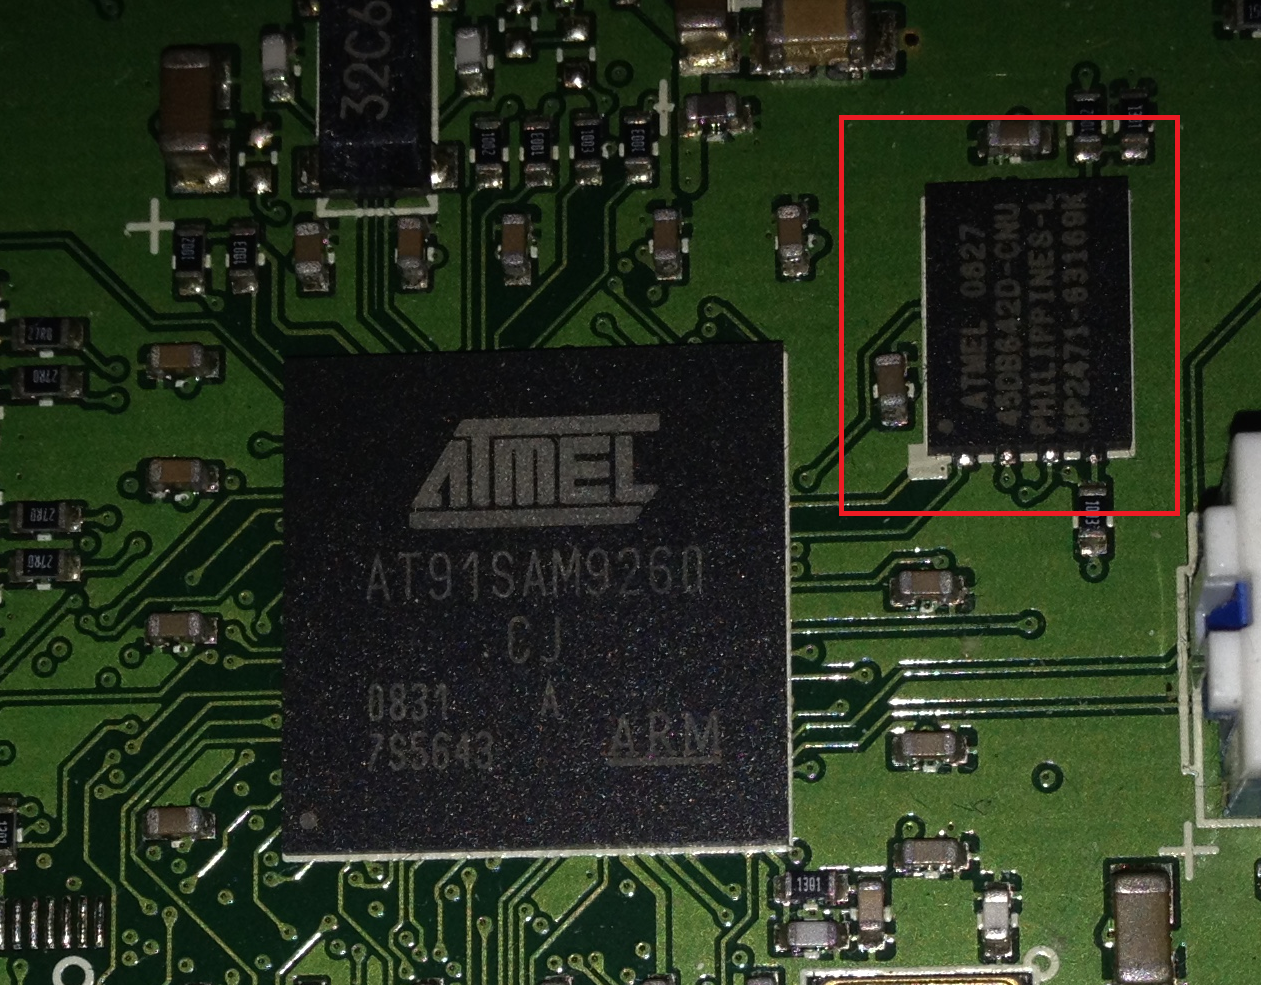
\includegraphics[width=0.5\textwidth]{Pictures/Flash}
		\caption{AT91SAM9260 processor and AT45DB642D DataFlash}
		\label{fig:Flash}
	\end{figure}
\subsection{Related Hardware}
\label{sec:related_hardware}
\par Based on the processor, specifications, and name, it is reasonable to assume that the DS9260 is a modification of KwikByte's KB9260 general-purpose single-board computer. The upshot of this is that slightly more documentation exists for the KB9260 than the DS9260. Specifically, KwikByte offers sample GPIO and ADC interface code for the KB9260 (\href{http://kwikbyte.com/KB9260/source/gpio.zip}{GPIO}, \href{http://kwikbyte.com/KB9260/source/adc.zip}{ADC}) which are also mirrored on carlosgj.org (\href{http://carlosgj.org/FRC/DS9260/gpio.zip}{GPIO}, \href{http://carlosgj.org/FRC/DS9260/adc.zip}{ADC}). These samples should, when compiled properly, run on the DS9260 as well (after modifying the \texttt{\#define}s to reflect the DS9260's pin mapping).
\subsection{Connection \& Communication}
\par Communication with the DS9260 takes place primarily over the DE9 ``competition port''. Despite appearances, this is not a plain serial port. While many of the pin functions are not yet know, basic RS232 serial capability is present on the normal pins: 2 (RX), 3 (TX), and 5 (ground). Therefore, a custom null-modem adapter was made which connects only those three pins. (The ``USB Adapter Clip'' from KwikByte was likely a similar connector, plus an FT232R chip for USB operation.)
\par Opening the serial port (115200, 8, N, 1) presents a banner and login prompt:
\begin{verbatim}
 --------------------
-                  -
- KwikByte DS9260  -
-                  -
- www.kwikbyte.com -
-                  -
--------------------
DS9260 login:
\end{verbatim}
While the root account is password protected, trial and error revealed a user account called ``default'' that did not require a  password. This allowed exploration of much of the filesystem. It appears to be a fairly standard embedded Linux system with BusyBox. The application software binaries are in /ds60x/bin, consisting of nine files: lcd, mgr\_joysx, recv\_pc, send\_fms, send\_robot, manager, recv\_fms, recv\_robot, and send\_pc.
\par For firmware updates and other pre-boot functionality, the normal boot process can be interrupted and a ``utility loader'' sent by serial as described in App. \ref{app:utilLoader}. This has basic facilities for memory read and write, as well as interaction with the SPI Flash memory.

\section{Dissection of Factory Image}
\par The first software item investigated was the image ``raw\_otb.bin'' provided by \href{http://www.kwikbyte.com/driverstation/binary/raw_otb.bin}{KwikByte} (also mirrored on \href{http://carlosgj.org/FRC/DS9260/raw_otb.bin}{carlosgj.org} for posterity).
\par This file is not a first-level bootloader, but is instead called from the kernel loader. As such, it is expected to contain at least the Linux kernel and an initrd. In fact, the most recognizable thing in the file is the Linux boot parameters at offset 0x58:
\begin{verbatim}
console=ttyS0,115200 root=/dev/ram rw initrd=0x22400000,851719 mem=64M
\end{verbatim}
\par The purpose of the preceeding data (including the string ``KwikByte'') and following data (mostly null bytes) is unknown. However, an educated guess would be that a compressed Linux kernel (zimage) exists in the file. Knowing that the zimage magic number, 0x016F2818, should be found at 0x24 from the beginning of the zimage, and finding this value at 0x443 in raw\_otb.bin, the zimage is expected to start at 0x420. Furthermore, based on the start and end addresses at 0x28 and 0x2C from the start of the zimage, respectively, the zimage is expected to end at 0x160494 of raw\_otb.bin. In order to examine the kernel image, the actual compressed kernel would have to be extracted (i.e., separated from the self-extraction code). Assuming the zimage uses gzip, the gzip ``magic number'', 0x1F8B, plus the expected compression method, 0x08, should be found (see the \href{https://tools.ietf.org/html/rfc1952}{gzip standard} for details). A search for 0x1F8B08 showed the first occurrence at offset 0x44F8. Metadata present in the gzip header reveals that the data was zipped on Fri, 03 Oct 2008 at 23:56:34 GMT on a Unix system. A partial copy of the raw\_otb.bin file from 0x44F8 to 0x160493 can indeed be unzipped, resulting in what appears to be a Linux kernel based on literal strings in the binary. In fact, one such string offers potentially valuable information:
\begin{verbatim}
Linux version 2.6.23DS60v1.0 (root@kbdev-laptop13) (gcc version 3.4.2) #7 
Fri Oct 3 16:56:31 MST 2008
\end{verbatim}
\par Just past the end of the kernel zimage, another occurrence of 0x1F8B08 is found, indicating the start of another archive. The metadata shows that it was zipped on Mon, 03 Nov 2008 at 20:23:39 GMT, with maximal compression, on a Unix system, and additionally that the original filename was ``initrd\_img''. Copying 0x160494 onwards results in another valid gzip, which successfully uncompresses into a filesystem.

\section{Gaining Root Access}
\par As a first step towards repurposing the DS9260, root access was needed to more thoroughly explore the system. First, on the host computer (running Debian Jessie), the \texttt{gunzip}ped initrd was mounted. Then, the root entry in /etc/shadow was edited to remove the password, resulting in:
\begin{verbatim}
root::10933:0:99999:7:::
bin:*:10933:0:99999:7:::
daemon:*:10933:0:99999:7:::
adm:*:10933:0:99999:7:::
lp:*:10933:0:99999:7:::
sync:*:10933:0:99999:7:::
shutdown:*:10933:0:99999:7:::
halt:*:10933:0:99999:7:::
uucp:*:10933:0:99999:7:::
operator:*:10933:0:99999:7:::
nobody:*:10933:0:99999:7:::
default::10933:0:99999:7:::
\end{verbatim}
\par This ``rooted'' filesystem image was then \texttt{gzip}ped, making sure that the gzip header and parameters matched the original. Knowing that the compressed initrd begins at 0x160494 of raw\_otb.bin, and that raw\_otb.bin is written to Flash at 0x42000 (per App. \ref{app:utilLoader}), the rooted gzip was written to SPI at 0x1A2494 (0x42000+0x160494) using the Util Loader. This resulted in a working system with a root account which does not require a password. Surprisingly, although the rooted initrd was slightly larger than the original, the ``initrd=0x22400000,851719'' boot argument did not have to be changed. 
\par This allowed much more in-depth experimentation with the DS9260. For example, to easily move files on and off the device, a flash drive could be used. Any USB mass storage device plugged into the DS9260 is assigned \texttt{/dev/sda} (multiple mass storage devices are apparently not supported). Then, the drive could be accessed by:
\begin{verbatim}
mkdir temp
mount /dev/sda1 temp/
\end{verbatim}
Additionally, other devices (LCD framebuffer, joysticks, etc.) could be read from and written to. (See later sections for details on interacting with peripherals.)

\section{Memory Organization}
\par The following output during boot describe the major sections of memory in the SPI Flash:
\begin{verbatim}
[    2.750000] 0x00000000-0x00001080 : "BOOT1"
[    2.760000] 0x00001080-0x000413a0 : "BOOT2"
[    2.770000] 0x000413a0-0x00042000 : "PARAM"
[    2.770000] 0x00042000-0x00840000 : "RAW"
\end{verbatim}
These partitions are mounted to \texttt{/dev/mtd0} through \texttt{/dev/mtd3} at boot. After gaining root access to the kernel, these sections were copied to a USB flash drive for examination, with \texttt{dd if=/dev/mtd0 of=temp/mtd0.bin bs=1} etc. The \textsc{raw} partition begins at 0x42000, which, as described in App. \ref{app:utilLoader}, is where the raw\_otb.bin image is written. This is, therefore, where the kernel and filesystem are stored. In addition, in accordance with App. \ref{app:kernelLoader}, the ``altloader'' is programmed into Flash starting at 0x7FE000. Finally, the 1024-byte block starting at 0x83FBE0 contains the splash image shown on the LCD at boot, in monochrome bitmap format. The \textsc{param} partition is apparently unused, as it is blank (null bytes) except for ASCII string ``test'' at the beginning. As described in App. \ref{app:kernelLoader}, the ``kernel loader'' (possibly a version of Das U-Boot) is programmed at 0x1080, indicating that \textsc{boot2} is the second-stage bootloader. \textsc{boot1}, therefore, must the first-stage bootloader, responsible for initializing the processor on power-up and launching U-Boot. It is called ``CopyLoader64 DS60x1.0'' according to a string in its contents.

\section{Compilation of Application Software}
\par In order to use the DS9260 for anything other than its original application, it is necessary to compile new software for it. Luckily, as described in \S\ref{sec:related_hardware}, KwikByte provides example code for the related KB9260. As a proof-of-concept, the GPIO example was compiled to run on the DS9260.
\par First of all, it was necessary to elucidate which AT91SAM9260 pins (e.g., PIO[A, B, C][0-31]) routed to which user-accessible interface before attempting to interact with the GPIO. As mentioned in App. \ref{app:utilLoader}, ``...you should not set a system-defined input pin as an output as this could damage the Driver Station.'' The AT91SAM9260 pins for the auto/teleop, up, down, and select buttons were found to be PIOB20, PIOB21, PIOB25, and PIOB27, respectively, using the ``pin'' command in the Util Loader. 
\par In the name of safety, the gpio/main.c file was modified to remove all of the digital output, leaving just the digital input polling. In addition, the input pin was changed to PIOB20. After generating a basic buildroot configuration (just cross-compilation toolchain, no kernel, rootfs, or bootloader) and modifying gpio/Makefile to use the buildroot toolchain (App. \ref{app:gpio}), the gpio software was successfully compiled. After copying it to the DS9260 via flash drive, it did indeed print the state of the auto/teleop switch to the console.

\section{Digital And Analog Peripherals}
\section{Writing To The LCD}
\section{TL;DR: Quickstart Guide}

\newpage 
\begin{appendices}
	\section{Utility Loader \& Firmware Update Instructions}
		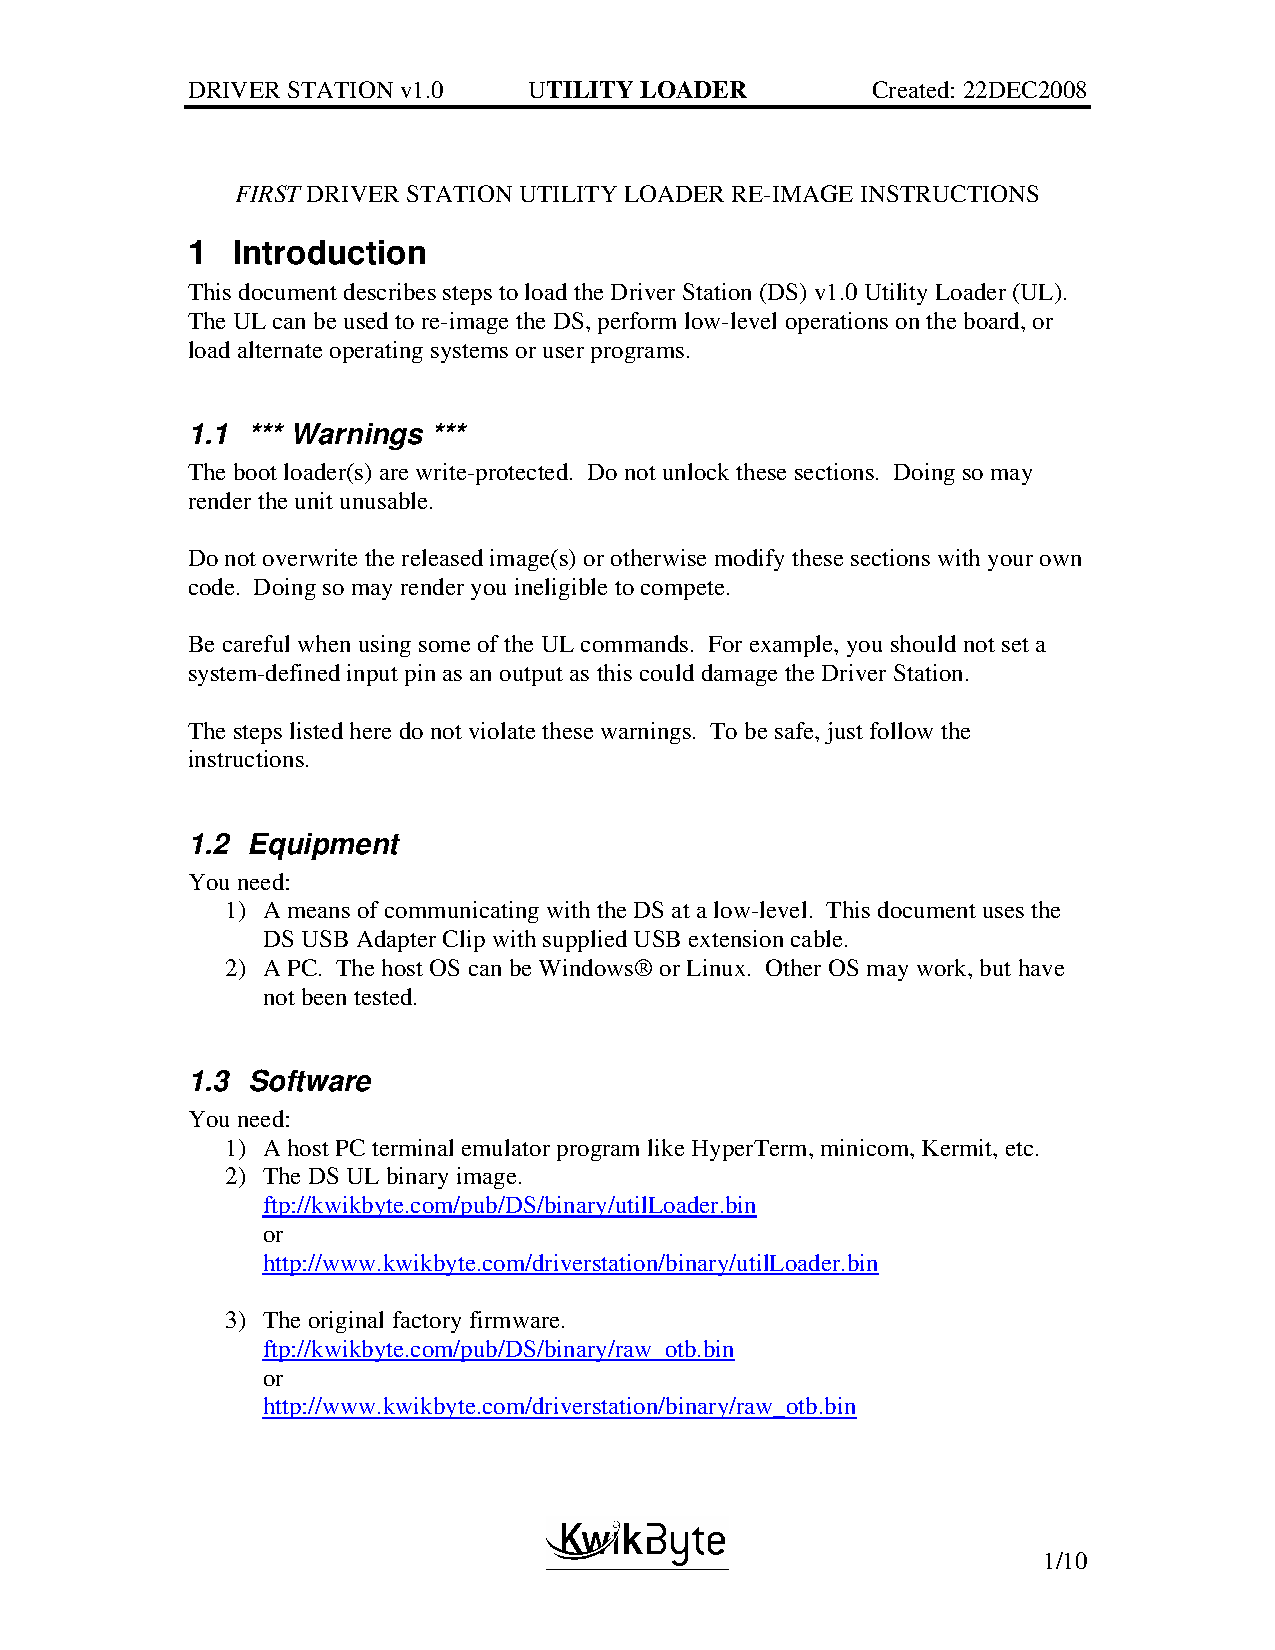
\includepdf[pages=-]{DS_utility_loader}
		\label{app:utilLoader}
	\section{Kernel Loader Update Instructions}
		\label{app:kernelLoader}
		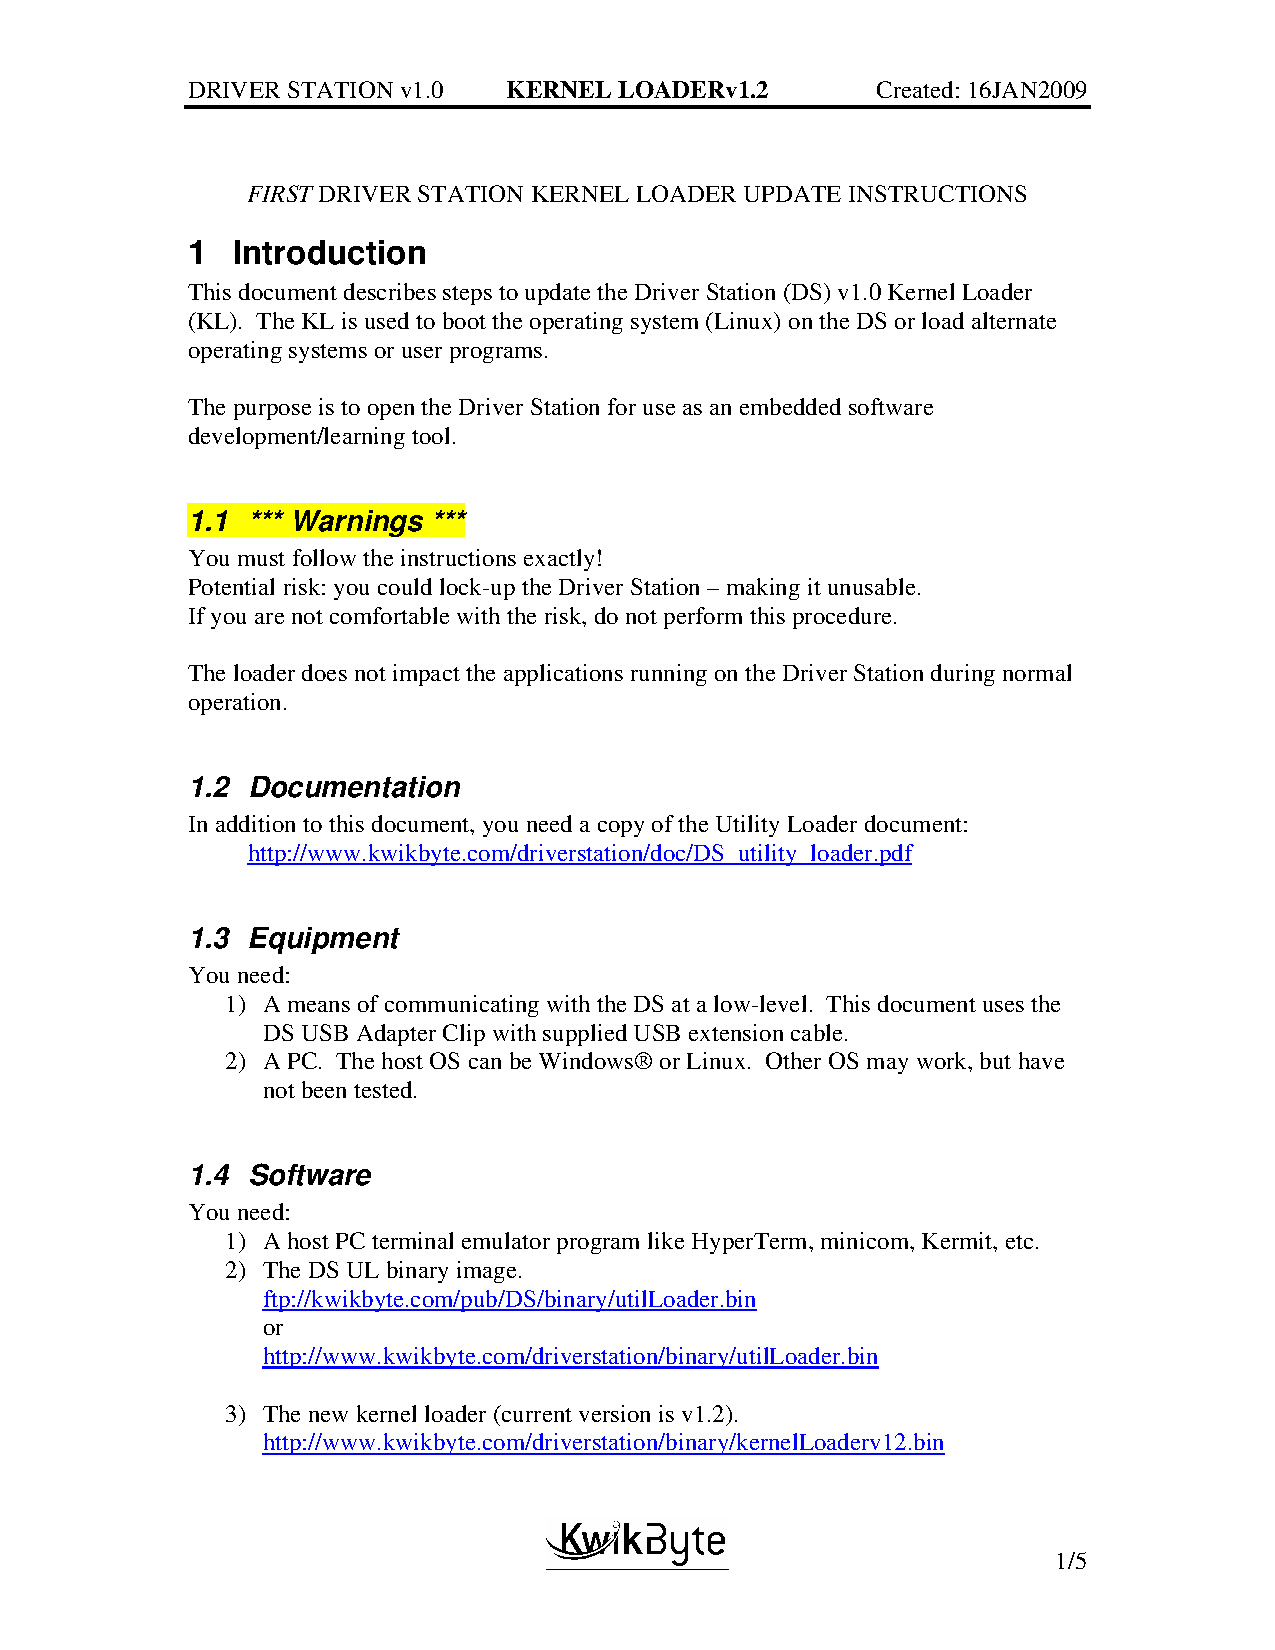
\includepdf[pages=-]{DS_kernelLoaderv12}
	\section{Logo Update Instructions}
		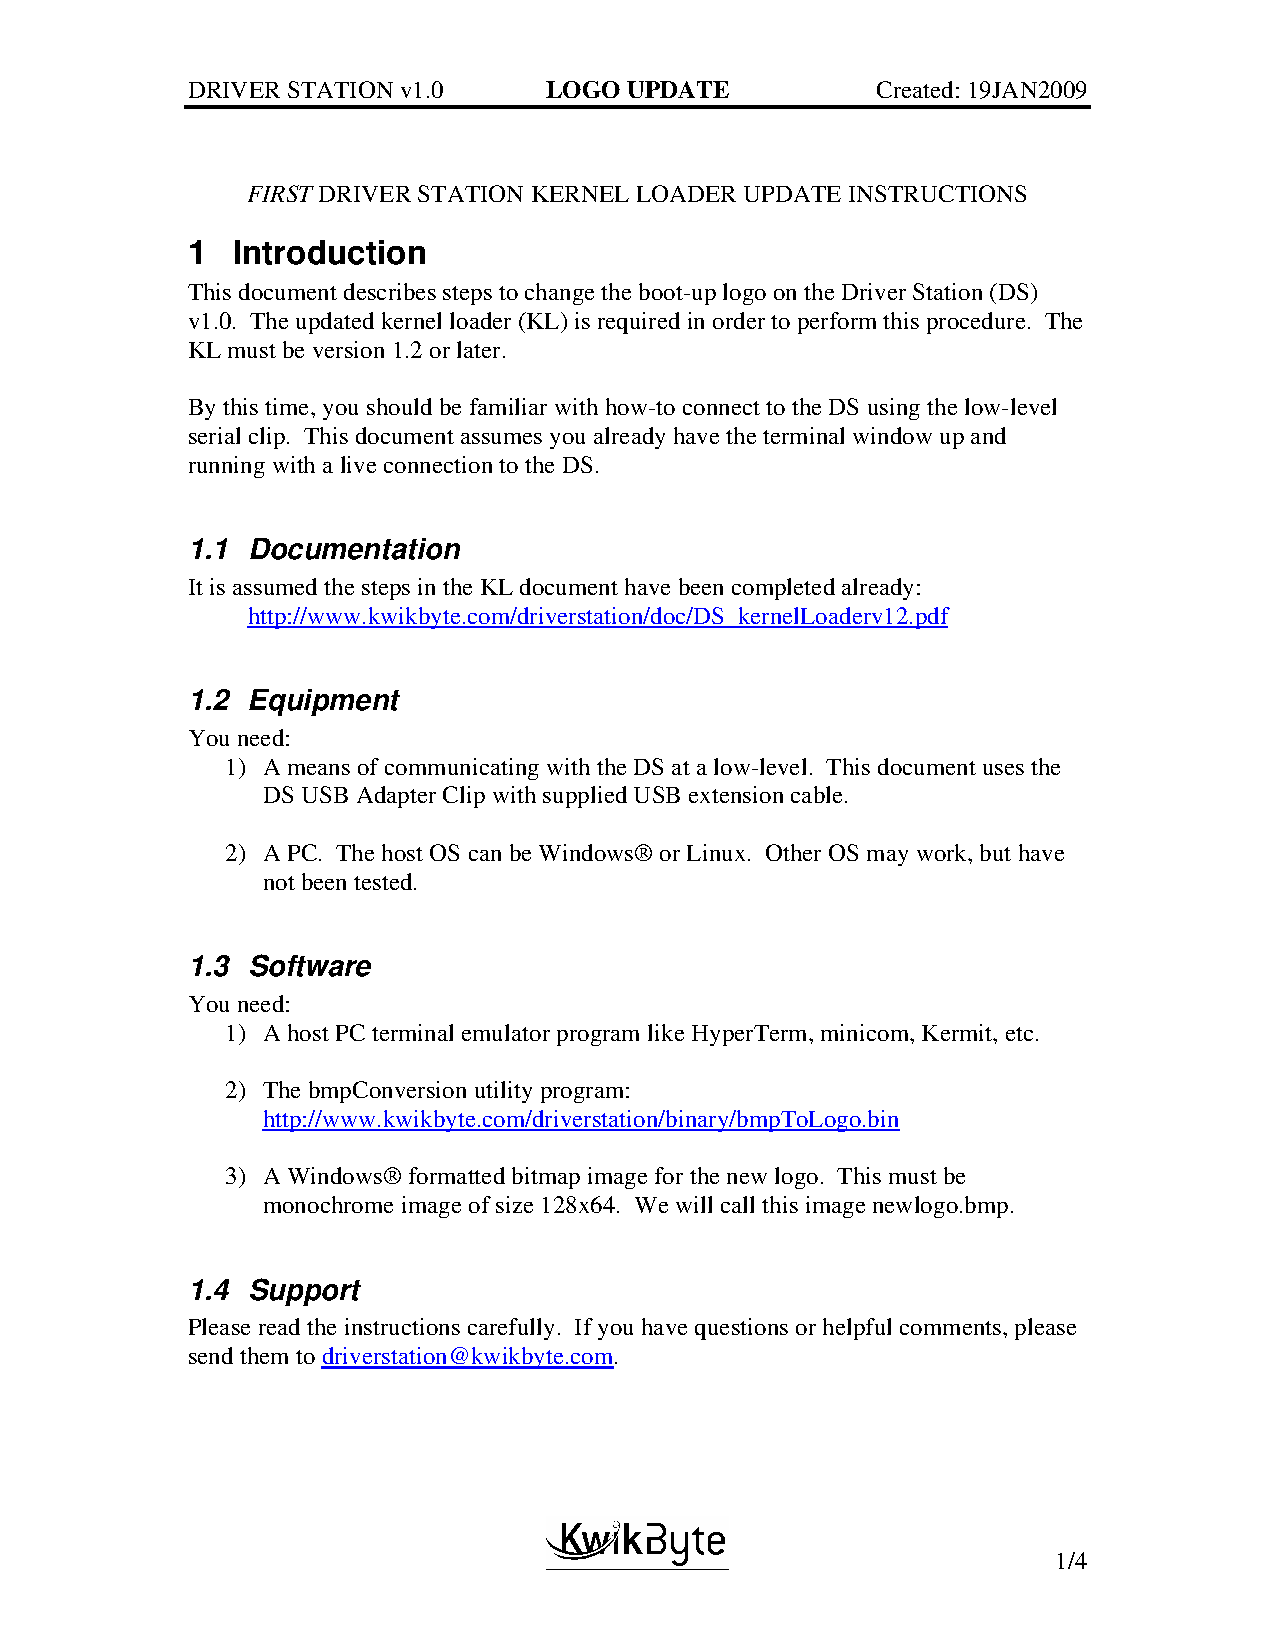
\includepdf[pages=-]{DS_logoUpdate}
	\section{Working GPIO Test}
		\label{app:gpio}
		\subsection{main.c}
		\verbatiminput{gpio/main.c}
		\subsection{Makefile}
		\verbatiminput{gpio/Makefile.txt}
		
\end{appendices}

\end{document}
